%%%%%%%%%%%%%%%%%%%%%%%%%%%%%%%%%%%%%%%%%
% Beamer Presentation
% LaTeX Template
% Version 1.0 (10/11/12)
%
% This template has been downloaded from:
% http://www.LaTeXTemplates.com
%
% License:
% CC BY-NC-SA 3.0 (http://creativecommons.org/licenses/by-nc-sa/3.0/)
%
%%%%%%%%%%%%%%%%%%%%%%%%%%%%%%%%%%%%%%%%%

%----------------------------------------------------------------------------------------
%	PACKAGES AND THEMES
%----------------------------------------------------------------------------------------

\documentclass{beamer}

\mode<presentation> {

	% The Beamer class comes with a number of default slide themes
	% which change the colors and layouts of slides. Below this is a list
	% of all the themes, uncomment each in turn to see what they look like.

	%\usetheme{default}
	%\usetheme{AnnArbor}
	%\usetheme{Antibes}
	%\usetheme{Bergen}
	%\usetheme{Berkeley}
	%\usetheme{Berlin}
	%\usetheme{Boadilla}
	%\usetheme{CambridgeUS}
	%\usetheme{Copenhagen}
	%\usetheme{Darmstadt}
	%\usetheme{Dresden}
	%\usetheme{Frankfurt}
	%\usetheme{Goettingen}
	%\usetheme{Hannover}
	%\usetheme{Ilmenau}
	%\usetheme{JuanLesPins}
	%\usetheme{Luebeck}
	%\usetheme{Madrid}
	%\usetheme{Malmoe}
	%\usetheme{Marburg}
	%\usetheme{Montpellier}
	%\usetheme{PaloAlto}
	\usetheme{Pittsburgh}
	%\usetheme{Rochester}
	%\usetheme{Singapore}
	%\usetheme{Szeged}
	%\usetheme{Warsaw}

	% As well as themes, the Beamer class has a number of color themes
	% for any slide theme. Uncomment each of these in turn to see how it
	% changes the colors of your current slide theme.

	%\usecolortheme{albatross}
	\usecolortheme{beaver}
	%\usecolortheme{beetle}
	%\usecolortheme{crane}
	%\usecolortheme{dolphin}
	%\usecolortheme{dove}
	%\usecolortheme{fly}
	%\usecolortheme{lily}
	%\usecolortheme{orchid}
	%\usecolortheme{rose}
	%\usecolortheme{seagull}
	%\usecolortheme{seahorse}
	%\usecolortheme{whale}
	%\usecolortheme{wolverine}

	%\setbeamertemplate{footline} % To remove the footer line in all slides uncomment this line
	%\setbeamertemplate{footline}[page number] % To replace the footer line in all slides with a simple slide count uncomment this line

	%\setbeamertemplate{navigation symbols}{} % To remove the navigation symbols from the bottom of all slides uncomment this line
}

\usepackage{graphicx} % Allows including images
\usepackage{booktabs} % Allows the use of \toprule, \midrule and \bottomrule in tables
%\usepackage{ctex}
\usepackage{multicol}

\usepackage{fontspec}
\setsansfont{Calibri}[
    Path=Font/,
    Scale=0.9,
    Extension = .ttf,
    UprightFont=*-Regular,
    BoldFont=*-Bold,
    ItalicFont=*-Italic,
    BoldItalicFont=*-BoldItalic
    ]
\usepackage{unicode-math}

% \setmathfont{Libertinus Math} % 使用默认的数学字体或你偏好的数学字体 Latin Modern Math

\usepackage{ragged2e}
\justifying\let\raggedright\justifying %两端对齐
\usepackage{tikz}
\usetikzlibrary{positioning}
\usetikzlibrary{calc}
%----------------------------------------------------------------------------------------
%	TITLE PAGE
%----------------------------------------------------------------------------------------

\title[Asset Pricing]{\textbf{Asset Pricing}} % The short title appears at the bottom of every slide, the full title is only on the title page

\subtitle{3. CAPM \& CCAPM}

\author[Cheng Hang]{Cheng Hang} % Your name
\institute[DUFE] % Your institution as it will appear on the bottom of every slide, may be shorthand to save space
{School of Fintech \\
	Dongbei University of Finance \& Economics \\ % Your institution for the title page
	\medskip
	\textbf{chenghangch@qq.com}% Your email address
}
\date{\today} % Date, can be changed to a custom date




\AtBeginSection[]
{
	\begin{frame}{Content}
		\begin{columns}[t]
			\begin{column}{0.5\textwidth}
				\tableofcontents[sections={1-3},sectionstyle=show/shaded,subsectionstyle=show/shaded/hide]
			\end{column}
			\begin{column}{0.5\textwidth}
				\tableofcontents[sections={4-6},sectionstyle=show/shaded,subsectionstyle=show/shaded/hide]
			\end{column}
		\end{columns}
		\addtocounter{framenumber}{-1}
	\end{frame}
}

%----------------------------------------------------------------------------------------
%	Begin
%----------------------------------------------------------------------------------------

\begin{document}

\begin{frame}
	\titlepage % Print the title page as the first slide
\end{frame}


% \begin{frame}{Preview Material 1: SDF, CAPM}
% 	\begin{itemize}
% 		\item \href{https://www.sciencedirect.com/science/article/pii/S1574010203010227}{\textcolor{blue}{Campbell, John Y., 2003, Chapter 13 Consumption-based asset pricing, Handbook of the Economics of Finance (Elsevier)}}.
% 		\item Chapter 1, 9 in Book \textbf{Cochrane, John H., 2005, Asset Pricing: Revised Edition (Princeton University Press)}.
% 		\item Chapter 3, 4 in Book \textbf{Campbell, John Y, 2017, Financial Decisions and Markets: A Course in Asset Pricing (Princeton University Press).
% 		}
% 		\item Chapter 8 in Book \href{ https://doi.org/10.1002/9781118445112.stat07954}{\textcolor{blue}{Empirical Asset Pricing: The Cross Section of Stock Returns: An Overview}} for empirical method

% 	\end{itemize}
% \end{frame}

\section{Some Facts}

\begin{frame}{Some Facts}
	\begin{enumerate}
		\item The average real return on stock is high. 8.1\% at an annual rate (1947.2 to 1998.4).
            \item The average stock market return of China's stock market is 15.8\% yearly (1995-2024).
		\item The average riskless real interest rate is low. In the postwar U.S. data, the average real return on 3-month Treasury bills was 0.9\% per year.
		\item Real stock returns are volatile, with an annualized standard deviation of 15.6\% in U.S. data.
		\item The real interest rate is much less volatile.
		\item Real consumption growth is very smooth.
		\item Real consumption growth and real stock returns have a quarterly correlation of 0.23 in the U.S. data.
		\item Excess returns on U.S. stock over Treasury bills are highly forecastable. The log price-dividend ratio forecasts 10\% of the variance of the excess return at a 1-year horizon, 22\% at a 2-year horizon, and 38\% at a 4-year horizon.
	\end{enumerate}
\end{frame}

\begin{frame}{Two Questions}
	\begin{enumerate}
		\item Why is the average real stock return so high in relation to the average short-term real interest rate?
		\item Why is the volatility of real stock returns so high in relation to the volatility of the short-term real interest rate?

	\end{enumerate}
\end{frame}

\begin{frame}{Abstract of \textcolor{blue}{Cochrane(2011)}}

	\textbf{Discount-rate variation} \textcolor{red}{is the central organizing question of current asset-pricing research}. I survey facts, theories, and applications. Previously, we thought returns were unpredictable, with variations in price-dividend ratios due to variations in expected cash flows. Now, it seems all price-dividend variation corresponds to discount-rate variation. We also thought that the cross-section of expected returns came from the CAPM. Now we have a zoo of new factors. I categorize discount-rate theories based on central ingredients and data sources. Incorporating discount-rate variation affects finance applications, including portfolio theory, accounting, cost of capital, capital structure, compensation, and macroeconomics.

\end{frame}

\section{SDF}

\begin{frame}{Stochastic Discount Factor: Consumption-Based Model}
	Investor decides:
	\begin{itemize}
		\item Save
		\item Consumption
		\item Investment
	\end{itemize}

	Our basic pricing equation from \textbf{the first order condition of that decision}. These two should be equal:
	\begin{itemize}
		\item marginal utility loss of consuming a little less today and buying a little more of the asset
		\item the marginal utility gain of consuming a little more of the asset's payoff in the future
	\end{itemize}
	The asset's price should equal the expected discounted value of the asset's payoff, using the \textbf{investor's marginal utility} to \textbf{discount} the payoff.
\end{frame}

\begin{frame}{Stochastic Discount Factor: Consumption-Based Model}
	The value at time $ t $ of a \textit{payoff} $ x_{t+1} $. We find the value of this payoff by asking what it is worth to a typical investor. We model investors by a utility function defined
	over current and future values of consumption:
	\begin{align*}
		U(C_t,C_{t+1}) = u(C_t) + \beta E_t[u(C_{t+1})]
	\end{align*}
where $\beta$ is the time discount factor.

Please assume that the investor can \textbf{freely} buy or sell as much of the payoff $ x_{t+1} $ as he wishes, at a price $ p_t $. How much will he buy or sell?
\end{frame}

\begin{frame}{Stochastic Discount Factor: Basic Pricing Equation}
	Denote by $ e $ the original consumption level (if the investor bought none of the asset), and denote by $ \xi $ the amount of the asset he chooses to buy. Then, his problem is
	\begin{align*}
		max_{\xi } \quad u(C_t) + \beta E_t[u(C_{t+1})] \quad s.t.
	\end{align*}
	\begin{align*}
		C_t &= e_t - p_t \xi \\
		C_{t+1} &= e_{t+1} + x_{t+1}\xi
	\end{align*}
\end{frame}

\begin{frame}{Stochastic Discount Factor: Basic Pricing Equation}
	\begin{align*}
		max_{\xi } & \quad u(e_t - p_t \xi) + \beta E_t[u(e_{t+1} + x_{t+1}\xi)] \\
		&0 = - p_{t}{u}'(C_t) + E_{t} \left [ \beta {u}'(C_{t+1}) x_{t+1}\right ] \\
		& p_{t}{u}'(C_t) = E_{t} \left [ \beta {u}'(C_{t+1}) x_{t+1}\right ]
	\end{align*}
	or
	\begin{align}
		p_{t} = E_{t} \left [ \beta \frac{{u}'(C_{t+1})}{{u}'(C_t)}x_{t+1} \right ]
		\label{equ:assetpricing}
	\end{align}
	Equation \textcolor{blue}{(\ref{equ:assetpricing})} is the central asset pricing formula.
\end{frame}

\begin{frame}{Stochastic Discount Factor}
	define the \alert{\textit{stochastic discount factor}} $M_{t+1}$ as
	\begin{align*}
		M_{t+1} = \beta \frac{{u}'(C_{t+1})}{{u}'(C_t)}
	\end{align*}
	the basic pricing formula \textcolor{blue}{(\ref{equ:assetpricing})} can simply be expressed as
	\begin{align}
		p_{t} = \mathbb{E}_{t} \left [ M_{t+1}x_{t+1} \right ]
		\label{equ:assetpricing2}
	\end{align}
	The price always comes at $ t $, the payoff at $ t + 1 $, and the expectation is conditional on time-$ t $ information.
	\begin{align*}
		p = \mathbb{E}(Mx)
	\end{align*}
\end{frame}

\begin{frame}{Stochastic Discount Factor}
		We can rewrite $ 1 = \mathbb{E}(M R_f) =  \mathbb{E}(M)  R_f$, so $ R_f = \frac{1}{\mathbb{E}(M)} $.

		We can also rewrite $p=\mathbb{E}(m) \mathbb{E}(x)+\operatorname{cov}(m, x)$. Substituting the risk-free rate equation, we obtain

		\begin{equation*}
			p=\frac{E(x)}{R_f}+ \underbrace{\operatorname{cov}(m, x)}_{\text {risk adjustment}}
		\end{equation*}

	\begin{itemize}
		\item The correlation between the random components of the common discount factor $m$  and the asset-specific payoff $x$ generates asset-specific risk corrections.
		\item $m_{t+1} $ is also often called the \textit{marginal rate of substitution} or \textit{pricing kernel}.
	\end{itemize}
\end{frame}

\begin{frame}{Risk Adjustment}
	\begin{equation*}
		p=\frac{E(x)}{R_f}+\frac{\operatorname{cov}\left[\beta u^{\prime}\left(c_{t+1}\right), x_{t+1}\right]}{u^{\prime}\left(c_t\right)}
	\end{equation*}
\end{frame}




\begin{frame}{Stochastic Discount Factor}
	\begin{align}
		1 &= E (MR)\\
		\log \mathbb{E}_{t} X &=\mathbb{E}_{t} \log X+\frac{1}{2} \operatorname{Var}_{t} \log X, r = ln(R)\\
		0&=\mathbb{E}_{t} r_{i, t+1}+\mathbb{E}_{t} m_{t+1}+\left(\frac{1}{2}\right)\left[\sigma_{i}^{2}+\sigma_{m}^{2}+2 \sigma_{i m}\right]\label{equ:1}
	\end{align}
where
\begin{align*}
	\sigma^2_{i} &= \operatorname{Var}\left(r_{i, t+1}-\mathbb{E}_{t} r_{i, t+1}\right)\\
	\sigma^2_{m} &= \operatorname{Var}\left(m_{t+1}-\mathbb{E}_{t} m_{t+1}\right) \\
	\sigma_{im} &= \operatorname{Cov}\left(r_{i, t+1}-\mathbb{E}_{t} r_{i, t+1}, m_{t+1}-\mathbb{E}_{t} m_{t+1}\right)
\end{align*}
\end{frame}

\begin{frame}{Stochastic Discount Factor}

	\begin{equation}
	\begin{aligned}
		&r_{f, t+1}=-\mathbb{E}_{t} m_{t+1}-\frac{\sigma_{m}^{2}}{2} \\
		&\mathbb{E}_{t}\left[r_{i, t+1}-r_{f, t+1}\right]+\frac{\sigma_{i}^{2}}{2}=-\sigma_{im}\label{equ:sigmaim}
	\end{aligned}
	\end{equation}
\begin{itemize}
	\item The variance term on the left-hand side of Equation (\ref{equ:sigmaim}) is a \textbf{Jensen's Inequality} adjustment arising from the fact that we are describing expectations of log returns. In effect, this term converts the expected excess return from a geometric average to an arithmetic average. It would disappear if we rewrote the equation in terms of the log expectation of the ratio of gross simple returns:
	\begin{equation*}
		 \log \mathrm{E}_{t}\left[\left(1+R_{i, t+1}\right) /\left(1+R_{f, t+1}\right)\right]=-\sigma_{i m}
	\end{equation*}
	\item Equation says that the \textbf{risk premium} is determined by the
	\textbf{negative} of the \textit{covariance} of the asset with the stochastic discount factor.
\end{itemize}
\end{frame}

\begin{frame}{Sharpe Ratio}
    \begin{equation}
    \sigma_m \geqslant \frac{\mathrm{E}_t\left[r_{i, t+1}-r_{f, t+1}\right]+\sigma_i^2 / 2}{\sigma_i}
    \label{equ:sharpe}
    \end{equation}
    
Equation \textcolor{blue}{(\ref{equ:sharpe})} says that the standard deviation of the log stochastic discount factor must be greater than this Sharpe ratio for all assets $i$, that is, it must be greater than the maximum possible Sharpe ratio obtainable in asset markets.
\begin{itemize}
    \item Volatility of the \textbf{SDF} is bounded by any asset's Sharpe Ratio.
\end{itemize}

\end{frame}

\section{C-CAPM}

\begin{frame}{Consumption-based asset pricing with power utility}
	Considering a time-separable power utility function defined over aggregate consumption $ C_t $:
	\begin{equation}
        u(C_t)= \begin{cases}\frac{C_t^{1-\gamma}-1}{1-\gamma} & \text { if } \gamma \neq 1 \\ \ln (C_t) & \text { if } \gamma=1\end{cases}
        \end{equation}
where $ \gamma $ is the coefficient of relative risk aversion ($ \gamma > 0 $).

\begin{itemize}
    \item Key Properties:
        \begin{enumerate}
            \item \textbf{Constant Relative Risk Aversion}: The relative risk aversion (RRA) is given by $-\frac{C \cdot u^{\prime \prime}(C)}{u^{\prime}(C)}= \gamma$, which is constant across all levels of $C$. This means individuals with CRRA utility exhibit the same proportional aversion to risk regardless of their wealth.
            \item \textbf{Intertemporal Elasticity of Substitution (EIS)}: The EIS, which measures the responsiveness of consumption growth to changes in the interest rate, is $\frac{1}{\gamma}$. This inverse relationship links risk aversion and consumption-smoothing behavior.
            \item \textbf{Homotheticity}: CRRA preferences are homothetic, meaning the marginal rate of substitution does not change if consumption is scaled proportionally. This makes the utility function suitable for modeling growth economies.
        \end{enumerate}
\end{itemize}
\end{frame}

\begin{frame}{Consumption-based asset pricing with power utility}
    \begin{itemize}
	\item It is scale-invariant, so risk premia do not alter with aggregate wealth
	given constant return distributions.
	\item Investors with different levels of wealth but the same risk aversion coefficient have the same portfolio.
	\item The utility function is \textbf{restrictive} in that it imposes that the elasticity of intertemporal substitution or EIS, $ \psi $, is the reciprocal of the CRRA $ \gamma $.
        \item Marginal Rate of Substitution (\textbf{MRS}) is
        \begin{equation*}
\mathrm{MRS}=\frac{\partial U / \partial C_t}{\partial U / \partial C_{t+1}}=\frac{\beta^{-1} C_t^{-\gamma}}{C_{t+1}^{-\gamma}}=\beta^{-1}\left(\frac{C_{t+1}}{C_t}\right)^\gamma
\end{equation*}
\begin{equation*}
\psi=\frac{d (\ln \left(\frac{C_{t+1}}{C_t}\right))}{d \ln (\mathrm{MRS})}=\frac{1}{\gamma}
\end{equation*}
\end{itemize}
\end{frame}

\begin{frame}{Consumption-based asset pricing with power utility}
	The marginal utility is
	\begin{align*}
		U^{\prime}\left(C_{t}\right)=C_{t}^{-\gamma}
	\end{align*}
	The log stochastic discount factor is
	\begin{align*}
		M_{t+1}=\beta\left(C_{t+1} / C_{t}\right)^{-\gamma}
	\end{align*}
The SDF will be conditional \textbf{lognormal} if consumption is \textbf{conditionally lognormal}. We assume lognormality here but relax this assumption later. Then, the log SDF is
\begin{equation} \label{equ:logSDF}
	m_{t+1}=\log (\beta)-\gamma \Delta c_{t+1}
\end{equation}

\end{frame}


\begin{frame}{Consumption-based asset pricing with power utility}

We now assume that consumption and asset returns are jointly conditionally \alert{homoskedastic}. Substituting (\textcolor{blue}{\ref{equ:logSDF}}) into the lognormal version of the fundamental equation of asset pricing Equation (\textcolor{blue}{\ref{equ:1}}), we have
	\begin{align}
		0=\mathrm{E}_{t} r_{i, t+1}+\log \beta-\gamma \mathrm{E}_{t} \Delta c_{t+1}+\left(\frac{1}{2}\right)\left[\sigma_{i}^{2}+\gamma^{2} \sigma_{\Delta c}^{2}-2 \gamma \sigma_{i \Delta c}\right]
	\end{align}
\begin{itemize}
	\item $   \sigma_{c}^2 $ denotes the conditional variance of consumption
	growth, which under homoskedasticity equals the unconditional variance of log consumption innovations $\operatorname{Var}\left(c_{t+1}-\mathrm{E}_{t} c_{t+1}\right)  $.
	\begin{align*}
	\sigma_{c}^2 &= \operatorname{Var}\left(c_{t+1}-\mathrm{E}_{t} c_{t+1}\right) = \operatorname{Var}\left(c_{t+1}-c_t-E_t\left(c_{t+1}-c_t\right)\right)\\
 & =\operatorname{var}\left(\Delta c_{t+1}-E_t\left(\Delta c_{t+1}\right)\right)  =\sigma_{\Delta c}^2 
	\end{align*}

	\item $ \sigma_{ic} $ denotes the conditional covariance between log asset returns and consumption growth, which under homoskedasticity equals the unconditional covariance of innovations
	\begin{align*}
		 \sigma_{i \Delta c}  = \sigma_{ic} =   \operatorname{Cov}\left(r_{i, t+1}-\mathrm{E}_{t} r_{i, t+1}, c_{t+1}-\mathrm{E}_{t} c_{t+1}\right)
	\end{align*}
\end{itemize}
\end{frame}

\begin{frame}{Consumption-based asset pricing with power utility}
		Risk free rate in equation \textcolor{blue}{(\ref{equ:sigmaim})} becomes
	\begin{align}\label{equ:rf}
		r_{f, t+1}=-\log \beta+\gamma \mathrm{E}_{t} \Delta c_{t+1}-\frac{\gamma^{2} \sigma_{\Delta c}^{2}}{2}
	\end{align}
	\begin{itemize}
		\item Riskless real rate is \alert{linear} in expected consumption growth, with slope coefficient equal to the \alert{coefficient of relative risk aversion} ($\gamma$).
		\item The conditional variance of consumption growth has a \alert{negative} effect on the riskless rate which can be interpreted as a \textbf{precautionary savings effect}.
	\end{itemize}
\end{frame}


\begin{frame}
	Expected excess return in equation \textcolor{blue}{(\ref{equ:sigmaim})} becomes
	\begin{align}\label{equ:consumption}
		\mathrm{E}_{t}\left[r_{i, t+1}-r_{f, t+1}\right]+\frac{\sigma_{i}^{2}}{2}=\gamma \sigma_{ic}
	\end{align}
\begin{itemize}
	\item The log risk premium on any asset is the coefficient of relative risk aversion times the covariance of the asset return with consumption growth
	\item An asset with a high consumption covariance tends to have low returns when consumption is low, that is when the marginal utility of consumption is high. Such an asset is risky and commands a large risk premium.
\end{itemize}
\end{frame}

\begin{frame}{Three Puzzles: Equity Premium Puzzle (Mehra and Prescott (1985))}
	\begin{table} [!htbp]
		\centering
		\caption{Equity Premium Puzzle}
		\resizebox{110mm}{20mm}{
		\begin{tabular}{cccccccccc}
			\hline
			\text { Country } & \text { Sample period } & $ \overline{a e r}_{e} $ & $ \sigma\left(e r_{e}\right) $ & $ \sigma(m) $ & $ \sigma(\Delta c) $ & $ \rho\left(e r_{e}, \Delta c\right) $ & $ \operatorname{cov}\left(e r_{e}, \Delta c\right) $ &$  \text { RRA(1) } $ & $ \text { RRA(2) } $ \\
			\hline \text { USA } & 1947.2-1998.3 & 8.071 & 15.271 & 52.853 & 1.071 & 0.205 & 3.354 & 240.647 & 49.326 \\
			\text { AUL } & 1970.1-1998.4 & 3.885 & 22.403 & 17.342 & 2.059 & 0.144 & 6.640 & 58.511 & 8.421 \\
			\text { CAN } & 1970.1-1999.1 & 3.968 & 17.266 & 22.979 & 1.920 & 0.202 & 6.694 & 59.266 & 11.966 \\
			\text { FR } & 1973.2-1998.3 & 8.308 & 23.175 & 35.848 & 2.922 & -0.093 & -6.315 & <0 & 12.270 \\
			\text { GER } & 1978.4-1997.3 & 8.669 & 20.196 & 42.922 & 2.447 & 0.029 & 1.446 & 599.468 & 17.542 \\
			\text { ITA } & 1971.2-1998.1 & 4.687 & 27.068 & 17.314 & 1.665 & -0.006 & -0.252 & <0 & 10.400 \\
			\text { JAP } & 1970.2-1998.4 & 5.098 & 21.498 & 23.715 & 2.561 & 0.112 & 6.171 & 82.620 & 9.260 \\
			\text { NTH } & 1977.2-1998.3 & 11.421 & 16.901 & 67.576 & 2.510 & 0.032 & 1.344 & 849.991 & 26.918 \\
			\text { SWD } & 1970.1-1999.2 & 11.539 & 23.518 & 49.066 & 1.851 & 0.015 & 0.674 & 1713.197 & 26.501 \\
			\text { SWT } & 1982.2-1998.4 & 14.898 & 21.878 & 68.098 & 2.123 & -0.112 & -5.181 & <0 & 32.076 \\
			\text { UK } & 1970.1-1999.1 & 9.169 & 21.198 & 43.253 & 2.511 & 0.093 & 4.930 & 185.977 & 17.222 \\
			\text { USA } & 1970.1-1998.3 & 6.353 & 16.976 & 37.425 & 0.909 & 0.274 & 4.233 & 150.100 & 41.178 \\
			\hline
		\end{tabular}}
	\begin{minipage}{110mm}\tiny
		Note: $ \overline{a e r}_{e} $ is the average return multiplied by 400 to express it in annualized percentage points. $ \sigma\left(e r_{e}\right) $ is the annualized standard deviation of the excess log stock return. $ \sigma(\Delta c) $ reports the annualized standard deviation of consumption growth.  $ \rho\left(e r_{e}, \Delta c\right) $ reports the correlation between the excess log stock return and consumption growth. The column headed RRA(1) uses Equation (\alert{\ref{equ:consumption}}) directly, dividing the adjusted average excess return by the estimated covariance to get estimated risk aversion. The column headed RRA(2) sets the correlation of stock returns and consumption growth equal to 1 before calculating risk aversion.
	\end{minipage}
	\end{table}
\end{frame}

\begin{frame}{Equity Premium Puzzle}
	\begin{itemize}
		\item The equity premium puzzle is a robust phenomenon in international data.
		\item The coefficients of relative risk aversion in the RRA(1) column are generally extremely large. They are usually many times greater than 10, the maximum level considered plausible by \href{https://doi.org/10.1016/0304-3932(85)90061-3}{\textcolor{blue}{Mehra and Prescott (1985)}}.
		\item Even when one ignores the low correlation between stock returns and
		consumption growth and gives the model its best chance by setting the correlation to one, the RRA(2) column still has risk aversion coefficients above 10 in all countries except Australia and Japan.
	\end{itemize}
\end{frame}


\begin{frame}{Three Puzzles: Risk-Free Puzzle (Weil (1989))}
	\begin{table} [!htbp]
		\centering
		\caption{Risk Free Puzzle}
		\resizebox{110mm}{25mm}{
			\begin{tabular}{ccccccccc}
				\hline
				 Country  & Sample period  & $ \overline{r_{f}} $ & $\overline{\Delta c} $ &$ \sigma(\Delta c) $ &  RRA(1) &  TPR(1) & RRA(2) &  TPR(2)  \\

				\hline
				\text { USA } & 1947.2-1998.3 & 0.896 & 1.951 & 1.071 & 240.647 & -136.270 & 49.326 & -81.393 \\
				\text { AUL } & 1970.1-1998.4 & 2.054 & 2.071 & 2.059 & 58.511 & -46.512 & 8.421 & -13.880 \\
				\text { CAN } & 1970.1-1999.1 & 2.713 & 2.170 & 1.920 & 59.266 & -61.154 & 11.966 & -20.618 \\
				\text { FR } & 1973.2-1998.3 & 2.715 & 1.212 & 2.922 & <0 & \text { N/A } & 12.270 & -5.735 \\
				\text { GER } & 1978.4-1997.3 & 3.219 & 1.673 & 2.447 & 599.468 & 9757.265 & 17.542 & -16.910 \\
				\text { ITA } & 1971.2-1998.1 & 2.371 & 2.273 & 1.665 & <0 & \text { N/A } & 10.400 & -19.765 \\
				\text { JAP } & 1970.2-1998.4 & 1.388 & 3.233 & 2.561 & 82.620 & -41.841 & 9.260 & -25.735 \\
				\text { NTH } & 1977.2-1998.3 & 3.377 & 1.671 & 2.510 & 849.991 & 21349.249 & 26.918 & -18.769 \\
				\text { SWD } & 1970.1-1999.2 & 1.995 & 1.001 & 1.851 & 1713.197 & 48590.956 & 26.501 & -12.506 \\
				\text { SWT } & 1982.2-1998.4 & 1.393 & 0.559 & 2.123 & <0 & \text { N/A } & 32.076 & 6.636 \\
				\text { UK } & 1970.1-1999.1 & 1.301 & 2.235 & 2.511 & 185.977 & 676.439 & 17.222 & -27.838 \\
				\text { USA } & 1970.1-1998.3 & 1.494 & 1.802 & 0.909 & 150.100 & -175.916 & 41.178 & -65.701 \\
				\hline
		\end{tabular}}
	\begin{minipage}{110mm}\tiny
		The table first shows the average risk-free rate, the mean consumption growth rate, and the standard deviation of consumption growth. These moments and the risk aversion coefficients calculated in the last Table are substituted into Equation (\alert{\ref{equ:rf}}), and the equation is solved for an implied time preference rate. The time preference rate is reported in percentage points per year; it can be interpreted as the riskless real interest rate that would prevail if consumption were known to be constant forever at its current level, with no growth and no volatility.
	\end{minipage}
	\end{table}
\end{frame}

\begin{frame}{Risk-Free Rate Puzzle}
	\href{https://doi.org/10.1016/0304-3932(89)90028-7}{\textcolor{blue}{Weil (1989)}}: The Equity Premium Puzzle and the Risk-Free Rate Puzzle
	\begin{itemize}
		\item To explain the \textbf{equity premium puzzle}, we need high risk aversion ($\gamma \approx 50$)
		\item But high $\gamma$ implies a \alert{very high} risk-free rate (investors want to borrow against future consumption growth)
		\item \textbf{Data}: Average real risk-free rate $\approx 1\%$ per year
		\item \textbf{Model prediction}: With $\gamma = 50$, $R_f$ should be $\approx 20\%$ or higher
	\end{itemize}
\end{frame}

\begin{frame}[allowframebreaks]{Responses to the Puzzles}
	\begin{itemize}
		\item Sampling error
		\begin{itemize}
			\item \href{https://doi.org/10.1111/j.1540-6261.1995.tb04039.x}{\textcolor{blue}{Brown, Goetzmann, and Ross (1995, JF)}}: Survival
		\end{itemize}
		\item Sample selection (Survivorship bias)
		\begin{itemize}
			\item \href{https://doi.org/10.1111/0022-1082.00133}{\textcolor{blue}{Jorion and Goetzmann (1999, JF)}}: Global stock markets
		\end{itemize}
		\item Mismeasurement of returns
		\begin{itemize}
			\item \href{https://doi.org/10.2469/faj.v48.n1.28}{\textcolor{blue}{Siegel (1992, FAJ)}}: Historical stock returns
		\end{itemize}
		\item Mismeasurement of consumption
		\begin{itemize}
			\item \href{https://doi.org/10.1086/426042}{\textcolor{blue}{Parker and Julliard (2005, JPE)}}: Ultimate consumption risk
			\item \href{https://doi.org/10.1111/j.1540-6261.2006.00848.x}{\textcolor{blue}{Yogo (2006, JF)}}: Durable consumption
		\end{itemize}
		\item Long-run consumption covariances
		\begin{itemize}
			\item \href{https://doi.org/10.1086/588200}{\textcolor{blue}{Hansen, Heaton, and Li (2008, JPE)}}
		\end{itemize}
		\item Rare disasters
		\begin{itemize}
			\item \href{https://doi.org/10.1016/0304-3932(88)90172-9}{\textcolor{blue}{Rietz (1988, JME)}}: Original idea
			\item \href{https://doi.org/10.1162/qjec.121.3.823}{\textcolor{blue}{Barro (2006, QJE)}}: Calibration with historical disasters
			\item \href{https://doi.org/10.1093/qje/qjs001}{\textcolor{blue}{Gabaix (2012, QJE)}}: Variable rare disasters
		\end{itemize}
		\item \textbf{Epstein-Zin preferences}
		\begin{itemize}
			\item \href{https://doi.org/10.2307/1913778}{\textcolor{blue}{Epstein and Zin (1989, Econometrica)}}
			\item \href{https://www.journals.uchicago.edu/doi/10.1086/261750}{\textcolor{blue}{Epstein and Zin (1991, JPE)}}
		\end{itemize}
		\item Ambiguity aversion
		\begin{itemize}
			\item \href{https://doi.org/10.1006/jeth.1995.1065}{\textcolor{blue}{Epstein and Wang (1995, JET)}}
			\item \href{https://doi.org/10.1093/rfs/hhh003}{\textcolor{blue}{Maenhout (2004, RFS)}}
		\end{itemize}
		\item Long-run risks
		\begin{itemize}
			\item \href{https://doi.org/10.1111/j.1540-6261.2004.00670.x}{\textcolor{blue}{Bansal and Yaron (2004, JF)}}: Seminal paper
			\item \href{https://doi.org/10.1016/j.jmoneco.2016.07.003}{\textcolor{blue}{Bansal, Kiku, and Yaron (2016, JME)}}: Empirical evidence
		\end{itemize}
		\item Habit formation
		\begin{itemize}
			\item \href{https://doi.org/10.1086/261693}{\textcolor{blue}{Constantinides (1990, JPE)}}: Internal habit
			\item \href{https://doi.org/10.1086/250059}{\textcolor{blue}{Campbell and Cochrane (1999, JPE)}}: External habit
		\end{itemize}
		\item Nonseparable utility

		\item Uninsurable idiosyncratic risk

		\item Portfolio restrictions (Limited participation)

	\end{itemize}
\end{frame}


%% ============================================
%% Part: From Discount Factors to Beta Representations
%% ============================================

\section{Payoff‐Based Factors (Beta and Alpha)}\label{beta}

\begin{frame}{Motivation: The Measurement Problem}
	\textbf{Challenge}: The true SDF $m$ depends on unobservable economic variables
	\begin{itemize}
		\item Consumption growth is measured with error, noise, and lag
		\item Macroeconomic data available only at low frequency (quarterly/annual)
		\item Marginal utility, preferences, and beliefs are fundamentally unobservable
	\end{itemize}
	
	\vspace{8pt}
	\textbf{Solution}: Use \alert{traded payoffs} (returns) to proxy for the SDF
	\begin{itemize}
		\item Returns are directly observable in financial markets
		\item High-frequency data (daily/monthly) enables precise estimation
		\item Tradability ensures economic relevance
	\end{itemize}
	
	\vspace{8pt}
	\begin{block}{Key Idea}
		Project the abstract SDF onto the space of traded assets to obtain a \textbf{payoff-based discount factor} that prices all assets correctly.
	\end{block}
\end{frame}

\begin{frame}{From SDF to Beta Representation: Basic Derivation}
	Start with the fundamental pricing equation:
	\begin{align*}
		1 &= E(mR^i) = E(m)E(R^i) + \text{cov}(m, R^i)
	\end{align*}
	
	Rearranging:
	\begin{align*}
		E(R^i) &= \frac{1}{E(m)} - \frac{\text{cov}(m, R^i)}{E(m)} \\[6pt]
		&= \frac{1}{E(m)} + \underbrace{\frac{\text{cov}(m, R^i)}{\text{var}(m)}}_{\beta_{i,m}} \cdot \underbrace{\left(-\frac{\text{var}(m)}{E(m)}\right)}_{\lambda_m}
	\end{align*}
	
	\vspace{5pt}
	\begin{block}{Beta Pricing Form}
		\vspace{-8pt}
		\begin{equation*}
			E(R^i) - R^f = \beta_{i,m} \cdot \lambda_m
		\end{equation*}
		where $\beta_{i,m}$ = amount of risk (exposure), $\lambda_m$ = price of risk (premium per unit)
	\end{block}
\end{frame}

\begin{frame}{Projecting $m$ onto Traded Payoffs}
	\textbf{The Projection Theorem}: Let $X$ be the space of traded payoffs. 
 
 Define:
	\begin{equation*}
		x^* = \text{proj}(m \mid X)
	\end{equation*}
	
	Then we can decompose:
	\begin{equation*}
		m = x^* + \varepsilon, \quad \text{where } E(\varepsilon R^i) = 0 \text{ for all } R^i \in X
	\end{equation*}
	
	\vspace{5pt}
	\textbf{Key Insight}: $x^*$ prices all traded assets correctly:
	\begin{align*}
		E(mR^i) = E(x^*R^i) + \underbrace{E(\varepsilon R^i)}_{=0} = E(x^*R^i) = 1
	\end{align*}
	
	\vspace{5pt}
	\begin{itemize}
		\item $x^*$ is a \alert{valid SDF} within the space of traded assets
		\item $x^*$ is itself a payoff (linear combination of returns)
		\item The pricing error $\varepsilon$ is orthogonal to all tradeable payoffs
	\end{itemize}
\end{frame}

\begin{frame}{Main Theorem: Payoff-Based Beta Representation}
	\begin{theorem}
		The pricing equation $1 = E(mR^i)$ implies an expected return-beta model:
		\begin{equation*}
			E(R^i) = \gamma + \beta_{i,x^*} \cdot \lambda_{x^*}
		\end{equation*}
		where $x^* = \operatorname{proj}(m \mid X)$ serves as the pricing factor.
		
		\vspace{8pt}
		Equivalently, using the return on $x^*$: let $R^* \equiv x^*/E(x^{*2})$, then
		\begin{equation*}
			E(R^i) = \gamma + \beta_{i,R^*} \cdot [E(R^*) - \gamma]
		\end{equation*}
	\end{theorem}
	
	\vspace{5pt}
	\textbf{Interpretation}:
	\begin{itemize}
		\item $\beta_{i,x^*}$: Sensitivity of asset $i$ to the payoff factor $x^*$
		\item $\lambda_{x^*}$: Market price of risk associated with $x^*$
		\item $R^*$: The return on the mimicking portfolio for $m$
	\end{itemize}
\end{frame}

\begin{frame}{Proof: Beta Representation with $x^*$}
	Since $x^*$ prices all assets:
	\begin{align*}
		1 = E(x^* R^i) = E(x^*)E(R^i) + \text{cov}(x^*, R^i)
	\end{align*}
	
	Solving for $E(R^i)$:
	\begin{align*}
		E(R^i) &= \frac{1}{E(x^*)} - \frac{\text{cov}(x^*, R^i)}{E(x^*)} \\[8pt]
		&= \underbrace{\frac{1}{E(x^*)}}_{\gamma} + \underbrace{\frac{\text{cov}(x^*, R^i)}{\text{var}(x^*)}}_{\beta_{i,x^*}} \cdot \underbrace{\left(-\frac{\text{var}(x^*)}{E(x^*)}\right)}_{\lambda_{x^*}}
	\end{align*}
	
	\vspace{5pt}
	\begin{block}{Result}
		\vspace{-5pt}
		\begin{equation*}
			E(R^i) = \gamma + \beta_{i,x^*} \cdot \lambda_{x^*}
		\end{equation*}
	\end{block}
\end{frame}

\begin{frame}{Proof: Beta Representation with $R^*$}
	Define the return on $x^*$: $R^* = \dfrac{x^*}{E(x^{*2})}$, so $x^* = R^* \cdot E(x^{*2})$
	
	\vspace{5pt}
	Substituting into the pricing equation:
	\begin{align*}
		E(R^i) &= \frac{1}{E(x^*)} - \frac{\text{cov}(x^*, R^i)}{E(x^*)} \\[6pt]
		&= \frac{1}{E(R^*)E(x^{*2})} - \frac{\text{cov}(R^*, R^i) \cdot E(x^{*2})}{E(R^*) \cdot E(x^{*2})} \\[6pt]
		&= \frac{E(R^{*2})}{E(R^*)} - \frac{\text{cov}(R^*, R^i)}{E(R^*)}
	\end{align*}
	
	Note: $E(R^{*2}) = E\left(\dfrac{x^{*2}}{E(x^{*2})^2}\right) = \dfrac{1}{E(x^{*2})}$
\end{frame}

\begin{frame}{Proof: Beta Representation with $R^*$ (Continued)}
	Rearranging:
	\begin{align*}
		E(R^i) = \underbrace{\frac{E(R^{*2})}{E(R^*)}}_{\gamma} + \underbrace{\frac{\text{cov}(R^*, R^i)}{\text{var}(R^*)}}_{\beta_{i,R^*}} \cdot \underbrace{\left(-\frac{\text{var}(R^*)}{E(R^*)}\right)}_{\lambda_{R^*}}
	\end{align*}
	
	\vspace{5pt}
	For $R^*$ itself:
	\begin{align*}
		E(R^*) = \gamma - \frac{\text{var}(R^*)}{E(R^*)} \quad \Longrightarrow \quad \lambda_{R^*} = E(R^*) - \gamma
	\end{align*}
	
	\vspace{5pt}
	\begin{block}{Final Result}
		\vspace{-5pt}
		\begin{equation*}
			E(R^i) = \gamma + \beta_{i,R^*} \cdot [E(R^*) - \gamma]
		\end{equation*}
		The risk premium of any asset equals its beta times the excess return on $R^*$.
	\end{block}
\end{frame}

\begin{frame}{Why Payoff-Based Factors?}
	\begin{columns}[T]
		\column{0.48\textwidth}
		\textbf{Advantages}
		\begin{enumerate}
			\item \textbf{Observability}
			\begin{itemize}
				\item Returns measured precisely
				\item High-frequency data available
			\end{itemize}
			\item \textbf{Testability}
			\begin{itemize}
				\item Direct empirical validation
				\item Standard regression methods
			\end{itemize}
			\item \textbf{Consistency}
			\begin{itemize}
				\item $x^*$ prices all assets correctly
				\item Links theory to tradeable instruments
			\end{itemize}
		\end{enumerate}
		
		\column{0.48\textwidth}
		\textbf{Limitations}
		\begin{enumerate}
			\item \textbf{Economic interpretation}
			\begin{itemize}
				\item May not capture ``deep'' risks
				\item Preferences remain hidden
			\end{itemize}
			\item \textbf{Model uncertainty}
			\begin{itemize}
				\item Which factors to include?
				\item Factor zoo problem
			\end{itemize}
			\item \textbf{Spanning}
			\begin{itemize}
				\item $x^*$ only spans traded space
				\item Non-traded risks excluded
			\end{itemize}
		\end{enumerate}
	\end{columns}
	
	\vspace{8pt}
	\begin{block}{Bottom Line}
		Payoff-based models (CAPM, Fama-French) are empirically tractable; Consumption-based models (C-CAPM) reveal economic origins of risk premia.
	\end{block}
\end{frame}


%% ============================================
%% CAPM
%% ============================================

%% ============================================
%% Section: CAPM - The First Payoff-Based Factor Model
%% ============================================

\section{CAPM}

\begin{frame}{CAPM: The First Payoff-Based SDF Proxy}
	\textbf{Recall}: We want to proxy the unobservable SDF $m$ with traded payoffs.
	
	\vspace{8pt}
	\textbf{CAPM's Solution}: Use the \alert{market portfolio return} $R^W$ as the single factor:
	\begin{equation*}
		m_{t+1} = a + b \cdot R^W_{t+1}
	\end{equation*}
	
	\vspace{5pt}
	\begin{itemize}
		\item Credited to \href{https://doi.org/10.1111/j.1540-6261.1964.tb02865.x}{\textcolor{blue}{Sharpe (1964)}} and \href{https://doi.org/10.1111/j.1540-6261.1965.tb02930.x}{\textcolor{blue}{Lintner (1965)}}
		\item The first, most famous, and most widely used asset pricing model
		\item Ties the discount factor directly to aggregate wealth
	\end{itemize}
	
	\vspace{8pt}
	\begin{block}{Beta Representation}
		\vspace{-5pt}
		\begin{equation*}
			E(R^i) - R^f = \beta_{i,R^W} \cdot [E(R^W) - R^f]
		\end{equation*}
		where $\beta_{i,R^W} = \dfrac{\operatorname{Cov}(R^i, R^W)}{\operatorname{Var}(R^W)}$
	\end{block}
\end{frame}

\begin{frame}{The Market Portfolio: Theory vs. Practice}
	\textbf{Theoretical Definition}: $R^W$ = return on \textit{total wealth} (human capital + financial assets + real estate + ...)
	
	\vspace{8pt}
	\textbf{Empirical Challenge}:
	\begin{itemize}
		\item No good data on total wealth
		\item Human capital is non-tradeable and hard to measure
		\item Real estate, private equity often excluded
	\end{itemize}
	
	\vspace{8pt}
	\textbf{Common Proxies}:
	\begin{itemize}
		\item Value-weighted NYSE/AMEX/NASDAQ
		\item S\&P 500 Index
		\item CRSP value-weighted market return
	\end{itemize}
	
	\vspace{8pt}
	\begin{alertblock}{Roll's Critique (1977)}
		The true market portfolio is unobservable. Tests of CAPM are joint tests of the model and the market proxy.
	\end{alertblock}
\end{frame}

\begin{frame}{Derivation I: Two-Period Quadratic Utility}
	\textbf{Setup}: Investors maximize quadratic utility over two periods:
	\begin{equation*}
		U(c_t, c_{t+1}) = -\frac{1}{2}(c^* - c_t)^2 - \frac{\beta}{2} E[(c^* - c_{t+1})^2]
	\end{equation*}
	
	\vspace{5pt}
	\textbf{Step 1}: Marginal rate of substitution
	\begin{equation*}
		m_{t+1} = \beta \frac{u'(c_{t+1})}{u'(c_t)} = \beta \frac{(c^* - c_{t+1})}{(c^* - c_t)}
	\end{equation*}
	
	\vspace{5pt}
	\textbf{Step 2}: Budget constraint links consumption to wealth
	\begin{align*}
		c_{t+1} &= W_{t+1} = R^W_{t+1}(W_t - c_t)
	\end{align*}
	where $R^W_{t+1} = \sum_{i=1}^{N} w_i R^i_{t+1}$ is the portfolio return.
\end{frame}

\begin{frame}{Derivation I: Two-Period Quadratic Utility (Continued)}
	\textbf{Step 3}: Substitute consumption into the SDF:
	\begin{align*}
		m_{t+1} &= \beta \frac{c^* - R^W_{t+1}(W_t - c_t)}{c^* - c_t} \\[8pt]
		&= \underbrace{\frac{\beta c^*}{c^* - c_t}}_{a_t} - \underbrace{\frac{\beta(W_t - c_t)}{c^* - c_t}}_{b_t} R^W_{t+1}
	\end{align*}
	
	\begin{block}{Result}
		\begin{equation*}
			m_{t+1} = a_t - b_t R^W_{t+1}
		\end{equation*}
		The SDF is \alert{linear in the wealth portfolio return}, which is exactly the CAPM specification.
	\end{block}

	\textbf{Note}: Quadratic utility $\Rightarrow$ mean-variance preferences $\Rightarrow$ only mean and variance of returns matter.
\end{frame}

\begin{frame}{Derivation II: Mean-Variance Efficiency Approach}
	\textbf{Alternative Logic}: If portfolio $p$ is mean-variance efficient, what does this imply?

	Consider adjusting weight $w_i$ (financed by the risk-free asset):
	\begin{align*}
		\frac{dR_p}{dw_i} &= R_i - R_f \quad \text{(effect on mean)} \\[5pt]
		\frac{d\operatorname{Var}(R_p)}{dw_i} &= 2\operatorname{Cov}(R_i, R_p) \quad \text{(effect on variance)}
	\end{align*}

	\textbf{Key Ratio}: Marginal improvement in mean per unit increase in variance
	\begin{equation*}
		\frac{dR_p/dw_i}{d\operatorname{Var}(R_p)/dw_i} = \frac{R_i - R_f}{2\operatorname{Cov}(R_i, R_p)}
	\end{equation*}
	
	\vspace{5pt}
	\textbf{Efficiency Condition}: This ratio must be \alert{identical for all assets} $i$.
\end{frame}

\begin{frame}{Derivation II: Why Must the Ratio Be Equal?}
	\textbf{Proof by Contradiction}: Suppose the ratios differ for assets $i$ and $j$.
	
	\vspace{8pt}
	Consider adjusting both weights to keep mean unchanged ($dR_p = 0$):
	\begin{equation*}
		dw_j = -\frac{(R_i - R_f)}{(R_j - R_f)} dw_i
	\end{equation*}
	
	\vspace{5pt}
	The change in variance is:
	\begin{equation*}
		d\operatorname{Var}(R_p) = \left[2\operatorname{Cov}(R_i, R_p) - 2\operatorname{Cov}(R_j, R_p)\frac{(R_i - R_f)}{(R_j - R_f)}\right]dw_i
	\end{equation*}
	
	\vspace{8pt}
	\textbf{If $d\operatorname{Var}(R_p) \neq 0$}: We could achieve lower variance with the same mean $\Rightarrow$ contradicts efficiency!
	
	\vspace{8pt}
	$\therefore$ For efficiency, we need $d\operatorname{Var}(R_p) = 0$, which requires:
	\begin{equation*}
		\frac{R_i - R_f}{2\operatorname{Cov}(R_i, R_p)} = \frac{R_j - R_f}{2\operatorname{Cov}(R_j, R_p)} \quad \text{for all } i, j
	\end{equation*}
\end{frame}

\begin{frame}{Derivation II: From Efficiency to Beta Pricing}
	Setting $j = p$ (the efficient portfolio itself):
	\begin{equation*}
		\frac{R_i - R_f}{2\operatorname{Cov}(R_i, R_p)} = \frac{R_p - R_f}{2\operatorname{Var}(R_p)}
	\end{equation*}
	
	\vspace{5pt}
	Rearranging:
	\begin{equation*}
		R_i - R_f = \frac{\operatorname{Cov}(R_i, R_p)}{\operatorname{Var}(R_p)}(R_p - R_f) = \beta_{ip}(R_p - R_f)
	\end{equation*}
	
	\vspace{8pt}
	\begin{block}{General Result}
		Any mean-variance efficient portfolio $p$ satisfies a beta pricing relation:
		\begin{equation*}
			E(R^i) - R_f = \beta_{ip}[E(R_p) - R_f]
		\end{equation*}
	\end{block}

	\textbf{CAPM's Assumption}: The \alert{market portfolio} $R^m$ is mean-variance efficient.
\end{frame}

\begin{frame}{The CAPM Equation}
	\textbf{Core Assumption}: In equilibrium, all investors hold the market portfolio, which must therefore be mean-variance efficient.
	
	\vspace{10pt}
	\begin{block}{The Capital Asset Pricing Model}
		\begin{equation*}
			E(R^i) - R_f = \beta_{im}[E(R^m) - R_f]
		\end{equation*}
		where $\beta_{im} \equiv \dfrac{\operatorname{Cov}(R^i, R^m)}{\operatorname{Var}(R^m)}$
	\end{block}
	
	\vspace{10pt}
	\textbf{Interpretation}:
	\begin{itemize}
		\item $\beta_{im}$: Systematic risk (exposure to market risk)
		\item $E(R^m) - R_f$: Market risk premium (price of risk)
		\item Only systematic risk is priced; idiosyncratic risk can be diversified away
	\end{itemize}
	
	\vspace{8pt}
	\textbf{Testable Prediction}: Expected returns are \alert{linear in market beta}, with zero intercept.
\end{frame}

\begin{frame}{Summary: Two Routes to CAPM}
	\begin{center}
		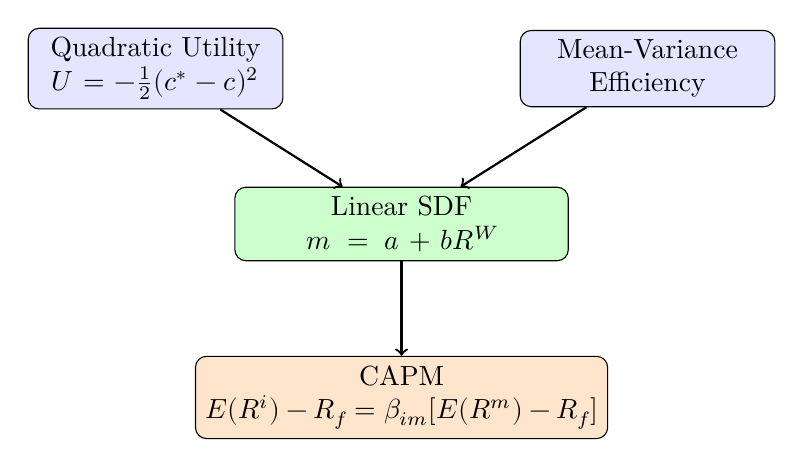
\begin{tikzpicture}[node distance=2cm, auto]
			% Nodes
			\node[draw, rounded corners, fill=blue!10, text width=3cm, align=center] (utility) {Quadratic Utility\\$U = -\frac{1}{2}(c^* - c)^2$};
			\node[draw, rounded corners, fill=blue!10, text width=3cm, align=center, right=3cm of utility] (mv) {Mean-Variance\\Efficiency};
			\node[draw, rounded corners, fill=green!20, text width=4cm, align=center, below=1.5cm of $(utility)!0.5!(mv)$] (sdf) {Linear SDF\\$m = a + bR^W$};
			\node[draw, rounded corners, fill=orange!20, text width=5cm, align=center, below=1.2cm of sdf] (capm) {CAPM\\$E(R^i) - R_f = \beta_{im}[E(R^m) - R_f]$};
			% Arrows
			\draw[->, thick] (utility) -- (sdf);
			\draw[->, thick] (mv) -- (sdf);
			\draw[->, thick] (sdf) -- (capm);
		\end{tikzpicture}
	\end{center}
	
	\vspace{5pt}
	\begin{itemize}
		\item \textbf{Route 1}: Preferences $\rightarrow$ Quadratic utility implies linear SDF in wealth return
		\item \textbf{Route 2}: Efficiency $\rightarrow$ MV-efficient portfolios satisfy beta pricing
		\item \textbf{Both routes}: Lead to the same testable prediction
	\end{itemize}
\end{frame}


\subsection{Empirical}

\begin{frame}{Testable Implications of the CAPM}
	\begin{enumerate}
		\item The CAPM predicts that cross-sectional variation in the expected returns of different securities is driven only by cross-sectional variation in the betas
		of the securities. \textbf{(This hypothesis is perhaps the most researched, and one of the most strongly refuted, hypotheses in all of empirical asset pricing.)}
		\begin{itemize}
			\item Examine the cross-sectional ability of beta to predict the future excess returns.
			\item Examines the cross-sectional ability of other variables to predict future excess returns. The CAPM predicts that no variable other than market beta should exhibit such predictive ability.
		\end{itemize}
	\item The average excess returns, after accounting for the effect of beta, should be zero. To test this hypothesis, researchers frequently examine the intercept term of cross-sectional regressions of security excess returns on beta estimates.
	\end{enumerate}
\end{frame}

\begin{frame}{Estimation of $ \beta $}
	 The most commonly used approach to estimating a stock’s market beta is to
	simply run a CAPM regression, also known as a one-factor market model regression.
	\begin{equation}\label{equ: CAPM}
		r_{i, t}=\alpha_{i}+\beta_{i} M K T_{t}+\epsilon_{i, t}
	\end{equation}
where $ r_{i, t} $ is the excess return of stock $ i $ during period $ t $, $ M K T_{t} $ is the excess return of the market portfolio (the market factor) during period $ t $, and $ \epsilon_{i, t} $ is the regression residual.
\end{frame}

\begin{frame}{Scholes and Williams (1977): nonsynchronous}
	\textbf{Scholes and Williams (1977)} present evidence that \textit{nonsynchronous} trading may affect empirical estimates of beta using the standard CAPM model. To account for this nonsynchronicity, they propose running a series of regressions
	\begin{align}
		r_{i, t} &=a_{i}+b_{i}^{-} M K T_{t-1}+e_{i, t}^{-} \\
		r_{i, t} &=a_{i}+b_{i} M K T_{t}+e_{i, t} \\
		r_{i, t} &=a_{i}+b_{i}^{+} M K T_{t+1}+e_{i, t}^{+}
	\end{align}
	and define $ \beta $ as
	\begin{align}
		\beta_{i}^{S W}=\frac{\hat{b}_{i}^{-}+\hat{b}_{i}+\hat{b}_{i}^{+}}{1+2 \rho}
	\end{align}
where $ \rho $ is the first-order serial correlation of the market portfolio's excess return.
\end{frame}

\begin{frame}{Dimson(1979): Infrequently Traded}
	\begin{align}
		\beta_{i}^{D}=\sum_{k=-5}^{k=5} \hat{b}_{i}^{k}
	\end{align}
where the $ \hat{b}_{i}^{k} $ are the estimated slope coefficients from the regression model
\begin{align}
	r_{i, t}=a_{i}+\sum_{k=-5}^{k=5} b_{i}^{k} M K T_{t+k}+e_{i, t}
\end{align}
\end{frame}


% \section{Factors Investment}

% \begin{frame}{Linear factor pricing models}
% 	\begin{itemize}
% 		\item The consumption-based model: a complete answer to most asset pricing questions in principle
% 		\item But is does not (yet) work well in practice
% 		\item  This observation motivates efforts to tie the discount factor $ m $ to other data.
% 	\end{itemize}
% 	Factor pricing models replace the consumption-based expression for marginal utility growth with a linear model of the form
% 	\begin{align*}
% 		m_{t+1}=a+b^{\prime} f_{t+1}
% 	\end{align*}
% \end{frame}

% \begin{frame}{Linear factor pricing models}
% 	\alert{The big question is, what should one use for factors $ f_{t+1} $?} \\
% 	Factor pricing models look for variables that are good proxies for aggregate marginal utility growth, i.e., variables for which
% 	\begin{align*}
% 		\beta \frac{u^{\prime}\left(c_{t+1}\right)}{u^{\prime}\left(c_{t}\right)} \approx a+b^{\prime} f_{t+1}
% 	\end{align*}
% \end{frame}

% \begin{frame}{Linear factor pricing models}
% 	\begin{itemize}
% 		\item In any sensible economic model, as well as in the data, consumption
% 		is related to returns on broad-based portfolios, to interest rates, to growth
% 		in GDP, investment, or other macroeconomic variables, and to returns on
% 		real production processes. All of these variables can measure the state of
% 		the economy.
% 		\item Consumption and marginal utility respond to news: if a
% 		change in some variable today signals high income in the future, then consumption rises now, by permanent income logic. This fact opens the door
% 		to \textit{forecasting} variables: \alert{Any variable that forecasts asset returns (changes in the investment opportunity set) or that forecasts macroeconomic variables is a candidate factor.} (term premium, dividend/price ratio, stock returns, etc.)
% 	\end{itemize}
% \end{frame}

% \begin{frame}{Ross(1976) Arbitrage Pricing Theory}
% 	\begin{align}
% 		E\left[R_{i}^{e}\right]=\beta_{i}^{\prime} \lambda
% 	\end{align}
% $ R_{i}^{e} $ is the stock \textbf{excess return}, $ \beta_{i} $ is\textbf{ factor exposure} or \textbf{factor loading}, $ \lambda $ is \textbf{factor expected return} or \textbf{factor risk premium}.

% \begin{align}
% 	E\left[R_{i}^{e}\right]=\alpha_{i}+\beta_{i}^{\prime} \lambda
% \end{align}
% $ \alpha_{i} $ is the pricing error of stock $i$ between the actual expected return rate of an asset and the expected return implied by the multi-factor model.

% \end{frame}

\section{CAPM fails}

\begin{frame}{Beta}
	\begin{itemize}
		\item The earliest empirical studies of the CAPM grouped stocks into portfolios using their historical market betas and found a positive and close to linear relationship between the subsequent betas of these portfolios and their average returns (\href{https://www.journals.uchicago.edu/doi/abs/10.1086/260061}{\textcolor{blue}{Fama and MacBeth(1973)}}).
		\item At the time, this was regarded as a success for
		the CAPM.
		\item Subsequent studies of the beta-return relationship have found an
		even weaker relationship between beta and return since the early 1960s, a period that tends to be much more challenging for the CAPM than the earlier part of the CRSP sample period.
	\end{itemize}
\end{frame}

\begin{frame}{Portfolio}
	\begin{table}[H]
		\tiny
		\caption{Univariate Portfolio Analysis—Equal-Weighte}
		\centering
		\resizebox{110mm}{20mm}{
			\begin{tabular}{ccccccccccccc}
				\hline Sort Variable & Coefficient & 1 & 2 & 3 & 4 & 5 & 6 & 7 & 8 & 9 & 10 & $10-1$ \\
				\hline\\
				 $\beta^{3 M}$ & $\beta^{3 M}$ & -0.62 & 0.01 & 0.23 & 0.42 & 0.59 & 0.78 & 0.98 & 1.23 & 1.58 & 2.41 & 3.04 \\
				 & Excess return & 0.74 & 0.76 & 0.85 & 0.79 & 0.83 & 0.80 & 0.80 & 0.76 & 0.68 & 0.43 & -0.30 \\
				 & & (2.18) & (2.79) & $(3.22)$ & (3.03) & $(3.21)$ & (2.89) & (2.74) & (2.39) & (1.95) & (1.02) & $(-1.37)$ \\
				 & CAPM $\alpha$ & 0.34 & 0.41 & 0.47 & 0.37 & 0.38 & 0.30 & 0.25 & 0.15 & -0.00 & -0.34 & -0.67 \\
				 & & (1.49) & $(2.39)$ & (3.03) & $(2.57)$ & (2.89) & $(2.19)$ & (1.78) & (1.05) & $(-0.00)$ & $(-1.31)$ & $(-2.85)$ \\
				\hline \\
				$\beta^{6 M}$ & $\beta^{6 M}$ & -0.32 & 0.12 & 0.30 & 0.47 & 0.62 & 0.78 & 0.96 & 1.18 & 1.48 & 2.14 & 2.46 \\
				 & Excess return & 0.84 & 0.76 & 0.84 & 0.84 & 0.84 & 0.81 & 0.74 & 0.78 & 0.62 & 0.37 & -0.47 \\
				 & & $(2.69)$ & $(2.94)$ & $(3.12)$ & $(3.23)$ & (3.15) & (2.86) & $(2.50)$ & (2.45) & (1.74) & $(0.87)$ & $(-1.97)$ \\
				 & CAPM $\alpha$ & 0.49 & 0.43 & 0.46 & 0.42 & 0.38 & 0.31 & 0.19 & 0.19 & -0.07 & -0.45 & -0.94 \\
				 & & $(2.25)$ & $(2.60)$ & $(2.84)$ & $(2.94)$ & (2.76) & $(2.12)$ & $(1.32)$ & $(1.12)$ & $(-0.43)$ & $(-1.93)$ & $(-4.13)$ \\
				\hline \\
				$\beta^{12 M}$ & $\beta^{12 M}$ & -0.13 & 0.18 & 0.35 & 0.50 & 0.64 & 0.79 & 0.95 & 1.15 & 1.42 & 1.98 & 2.11 \\
				 & Excess return & 0.92 & 0.87 & 0.91 & 0.85 & 0.86 & 0.87 & 0.77 & 0.65 & 0.60 & 0.38 & -0.53 \\
				 & & $(3.25)$ & $(3.36)$ & (3.38) & $(3.22)$ & $(3.22)$ & (3.08) & $(2.53)$ & (2.04) & (1.67) & $(0.91)$ & $(-2.04)$ \\
				 & CAPM $\alpha$ & 0.61 & 0.55 & 0.53 & 0.43 & 0.40 & 0.40 & 0.21 & 0.04 & -0.10 & -0.45 & -1.05 \\
				 & & $(3.05)$ & $(3.26)$ & $(3,28)$ & $(2.89)$ & $(2.74)$ & $(2.33)$ & $(1.41)$ & $(0.24)$ & $(-0.61)$ & $(-2.01)$ & $(-4.45$)\\
				\hline
			\end{tabular}
	}
	\end{table}

	You can see more details of $ \beta $ portfolios in Chapter 8 of Bali, Engle, and Murray (2017).
\end{frame}

\begin{frame}{Size}
	\begin{itemize}
		\item  \href{https://doi.org/10.1016/0304-405X(81)90018-0}{\textcolor{blue}{Banz(1981)}} found that firms with low market capitalization (``small" firms)
		tend to have higher average returns than their betas justify.
		\item But the size effect no longer commands so much attention for several reasons:
		\begin{enumerate}
			\item Large stocks outperformed small ones during the 1990s and part of the 2000s
			\item \href{https://www.sciencedirect.com/science/article/pii/0304405X83900259}{\textcolor{blue}{Keim(1983)}} and \href{https://www.sciencedirect.com/science/article/pii/0304405X83900296}{\textcolor{blue}{Reinganum (1983)}} pointed out that small stock outperformance was concentrated in \textit{January}, a seasonal anomaly that began to disappear shortly after it was publicized.
			\item \href{https://doi.org/10.1016/j.jfineco.2018.05.006}{\textcolor{blue}{Asness et al. (2018)}} found a significant size premium after you control the junk.
		\end{enumerate}
	\end{itemize}
\end{frame}


\begin{frame}{Value}
	\begin{itemize}
		\item \textbf{Value} investors seek to buy stocks with low market capitalization relative to accounting measures of their value, believing that such stocks will outperform.
		\item Academic studies have considered several alternative measures of value, including the dividend-price ratio or dividend yield, the earnings-price ratio
		(Basu 1977, 1983), and the book-market ratio. Since the influential work of \href{https://onlinelibrary.wiley.com/doi/10.1111/j.1540-6261.1992.tb04398.x}{\textcolor{blue}{Fama and French(1992)}}, \href{https://www.sciencedirect.com/science/article/pii/0304405X93900235}{\textcolor{blue}{Fama and French(1993)}}, attention now focuses mainly on the book-market ratio.
		\item During the last 50 years, ``value stocks" with high book-market ratios have had lower market betas than ``growth stocks" with low book-market ratios but higher average returns.
              \item \href{{https://www.jstor.org/stable/3694834}}{\textcolor{blue}{Zhang(2005)}} provides a groundbreaking explanation for this phenomenon within the neoclassical framework, emphasizing the roles of costly reversibility and countercyclical price of risk. 
	\end{itemize}
\end{frame}

% ---------------------------------------------------------
% 1. Momentum: The Premier Anomaly
% ---------------------------------------------------------
\begin{frame}{Momentum}
	\begin{itemize}
		\item \textbf{Momentum} is the tendency for assets that have performed well in the recent past to continue to perform well in the near future.
		\item \href{https://onlinelibrary.wiley.com/doi/10.1111/j.1540-6261.1993.tb04702.x}{\textcolor{blue}{Jegadeesh and Titman (1993)}} showed that a strategy of buying past winners (top decile) and selling past losers (bottom decile) generates significant positive abnormal returns that CAPM cannot explain.
		\item \textbf{Why it matters:} Momentum is robust across asset classes and countries (\href{https://doi.org/10.1111/jofi.12021}{\textcolor{blue}{Asness, Moskowitz, and Pedersen, 2013}}), yet it is difficult to explain with risk-based models.
		\item \textbf{Mechanisms:}
		\begin{enumerate}
			\item \textit{Behavioral:} Investor underreaction to news or overreaction due to self-attribution bias (\href{https://doi.org/10.1016/S0304-405X(98)00027-0}{\textcolor{blue}{Barberis, Shleifer, and Vishny, 1998}}; \href{https://onlinelibrary.wiley.com/doi/full/10.1111/0022-1082.00077}{\textcolor{blue}{Daniel, Hirshleifer, and Subrahmanyam, 1998}}).
			\item \textit{Risk-based:} Growth rate risk or varying expected returns (\href{https://onlinelibrary.wiley.com/doi/abs/10.1111/1540-6261.00431}{\textcolor{blue}{Johnson, 2002}}).
		\end{enumerate}
	\end{itemize}
\end{frame}

% ---------------------------------------------------------
% 2. Profitability: The "Quality" Dimension
% ---------------------------------------------------------
\begin{frame}{Profitability}
	\begin{itemize}
		\item More profitable firms earn significantly higher average returns than unprofitable firms.
		\item \href{https://doi.org/10.1016/j.jfineco.2013.01.003}{\textcolor{blue}{Novy-Marx (2013)}} identified that gross profitability has roughly the same power as book-to-market in predicting the cross-section of average returns.
		\item \textbf{The Puzzle:} Profitable firms are generally less prone to distress and have lower operating leverage, implying they should be \textit{safer} (lower CAPM beta) and earn \textit{lower} returns. The data shows the opposite.
		\item \textbf{Valuation Logic:}
		$$ P_t = \sum_{\tau=1}^{\infty} \frac{E_t(D_{t+\tau})}{(1+r)^\tau} $$
		Fixing current price $P_t$ and expected investment, higher expected profitability (proxied by dividends $D$) implies a higher discount rate $r$. This logic underpins the \href{https://doi.org/10.1016/j.jfineco.2014.10.010}{\textcolor{blue}{Fama and French (2015)}} 5-factor model.
	\end{itemize}
\end{frame}

% ---------------------------------------------------------
% 3. Investment: The Supply Side
% ---------------------------------------------------------
\begin{frame}{Investment (Asset Growth)}
	\begin{itemize}
		\item Firms with high asset growth or high investment rates tend to earn significantly lower subsequent returns.
		\item \href{https://doi.org/10.1111/j.1540-6261.2008.01370.x}{\textcolor{blue}{Cooper, Gulen, and Schill (2008)}} document a strong negative relation between total asset growth and future stock returns.
		\item \textbf{Mechanisms:}
		\begin{itemize}
			\item \textit{q-theory:} Given diminishing marginal returns to investment, firms invest more when their cost of capital ($r$) is low. Thus, high investment predicts low returns (\href{https://doi.org/10.1086/649760}{\textcolor{blue}{Liu, Whited, and Zhang, 2009}}; \href{https://doi.org/10.1093/rfs/hhu068}{\textcolor{blue}{Hou, Xue, and Zhang, 2015}}).
			\item \textit{Empire Building:} Managers overinvest due to agency problems, destroying shareholder value (\href{https://doi.org/10.1017/S0022109000003173}{\textcolor{blue}{Titman, Wei, and Xie, 2004}}).
		\end{itemize}
	\end{itemize}
\end{frame}

% ---------------------------------------------------------
% 4. Idiosyncratic Volatility: Challenging Diversification
% ---------------------------------------------------------
\begin{frame}{Idiosyncratic Volatility (IVOL)}
	\begin{itemize}
		\item According to the CAPM, idiosyncratic risk can be diversified away and should not be priced.
		\item \href{https://doi.org/10.1111/j.1540-6261.2006.00836.x}{\textcolor{blue}{Ang, Hodrick, Xing, and Zhang (2006)}} found a puzzling anomaly: stocks with high idiosyncratic volatility earn abysmally low average returns.
		\item This relationship is robust to controlling for size, book-to-market, momentum, and liquidity effects.
		\item \textbf{Potential Explanations:}
		\begin{itemize}
			\item \textit{Lottery Preferences:} Investors love positive skewness and overpay for volatile stocks that resemble lottery tickets (\href{https://doi.org/10.1257/aer.98.5.2066}{\textcolor{blue}{Barberis and Huang, 2008}}).
			\item \textit{Limits to Arbitrage:} Shorting high-IVOL stocks is costly and risky (\href{https://doi.org/10.1111/jofi.12286}{\textcolor{blue}{Stambaugh, Yu, and Yuan, 2015}}).
		\end{itemize}
	\end{itemize}
\end{frame}

\begin{frame}{Summary: Towards the Fama-French Three-Factor Model}
	\begin{itemize}
		\item \textbf{The Empirical Failure of CAPM:}
		The central prediction of the CAPM—that market beta is the sole measure of risk explaining average returns—is not supported by the data.
		\begin{itemize}
			\item The relationship between beta and average returns is too flat (\href{https://doi.org/10.1086/260061}{\textcolor{blue}{Fama and MacBeth, 1973}}).
			\item High beta stocks do not necessarily earn higher returns, and low beta stocks do not necessarily earn lower returns.
		\end{itemize}
		
		\item \textbf{Systematic Patterns (Anomalies):}
		Deviations from the CAPM are not random noise. Specific characteristics consistently predict returns:
		\begin{itemize}
			\item \textbf{Size:} Small firms outperform large firms (\href{https://doi.org/10.1016/0304-405X(81)90018-0}{\textcolor{blue}{Banz, 1981}}).
			\item \textbf{Value:} High Book-to-Market firms outperform low Book-to-Market firms (\href{https://doi.org/10.1111/j.1540-6261.1992.tb04398.x}{\textcolor{blue}{Fama and French, 1992}}).
		\end{itemize}
		
		\item \textbf{The Paradigm Shift:}
		\href{https://doi.org/10.1016/0304-405X(93)90023-5}{\textcolor{blue}{Fama and French (1993)}} synthesized these findings into a new standard. They argued that Size and Book-to-Market are not just ``anomalies'' but proxies for underlying risk factors (SMB and HML) related to financial distress.
		\item This paved the way for the \textbf{Fama-French Three-Factor Model}, which became the primary benchmark for empirical asset pricing for the next two decades.
	\end{itemize}
\end{frame}

\end{document}